\documentclass{article}
\usepackage{graphicx} % Required for inserting images
\usepackage[colorlinks=true, allcolors=blue]{hyperref}
\usepackage{titlesec}
\usepackage[square,numbers]{natbib}
\usepackage{geometry}
\geometry{
a4paper,
total={170mm,257mm},
left=20mm,
top=20mm,
}
\graphicspath{ {./images/} }

\bibliographystyle{dinat}

\title{Unit 23}
\author{Chris Hadden}
\date{}

\begin{document}

\maketitle
\section{D1 Evaluate the potential repurposing of your solution to other business sectors}
We will show in this report how our Patient Diagnosis chatbot that we defined in Task 4 P3 could be used in other areas so that we can be more efficent. This is called repurposing which is taking an existing technology and adapting it for another purpose.
\smallbreak

\section{Prior art}
Prior art is other projects or work that does the same thing that we are doing. You can find normally find it by searching on google with phrases that describe your own work. We are going to look for other healthcare chatbots on google search and see how they repurposed them.
\smallbreak
Noel Kennedy said that "A chatbot designed for the Healthcare industry to answer calls from the general public to their GP greatly improves the efficiency of obtaining appointments, getting sound medical advice and reduces the workload on the staff in the GP's surgery. Would this same technology be of use in the retail or finance sector to reduce call waiting times?" \cite{Noel}

This is a fair point.
\smallbreak

\subsection{Comparing Physician and Artificial Intelligence Chatbot Responses to Patient Questions Posted to a Public Social Media Forum}
The title in the heading\cite{bedside} said that "a chatbot generated quality and empathetic responses to patient questions posed in an online forum" and "Further exploration of this technology is warranted in clinical settings, such as using chatbot to draft responses that physicians could then edit". What it is saying is that the chatbot is easy to talk to and that all chatbots are like . This could make us think about using the chatbot as a therapist of some kind.


\subsection{Bookings}\label{booking}
One of the main uses of our chatbot is to make a booking to see GP. Looking in to chatbots that can make bookings there are lots of businesses that have already been setup to do that.\cite{futr}\cite{booking}\cite{velma} "In September 2017, Finnair launched its first chatbot via Facebook Messenger. Nicknamed Finn, it can sell flights, calculate how much baggage a passenger can take and respond to questions."\cite{booking} That is very advanced and shows that our chatbot could take on quite a lot.

\subsection{Expanding on diagnosis}
The chatbot main use was to help with diagnosis of the patient's and to making the GP's work quicker and easier. This is a perfect use of a chatbot in that it works with the GP and allows them to work with more patients.
Using this could be used in other areas where a client knows what the symptoms of a problem are. The chatbot could help to work out what the actual problem is. There's a number of chatbots that can already do this. \cite{gyan}\cite{devops}

\section{Assessing our chatbot}
Listing out the main features in our chatbot, and list them in importance. This will mean that we can find the chatbot's strengths and weaknesses and see if we can link them to the prior art to come up with any new creative applications for the chatbot.
\smallbreak
From best to worst theres:
\begin{enumerate}
    \item Bot can diagnose patient problems
    \item Bot saves time for GP
    \item Bot can take action on behalf of patient like making a booking
    \item Bot can be empathetic
    \item Bot may be seen as soulless
    \item Bot may make incorrect diagnosis and as such needs to be monitored
    \item Bot may remove certain jobs, and those employees may not be able to or unwilling to retrain
\end{enumerate}

\subsection{Bot can diagnose patient problems / Bot saves time for GP} \label{diagnose}

This is vthe best thing of our chat bot. The diagnosis is something that can be reused in other places. 
When working out whats going wrong with something would be a bit like this.
\begin{center} 
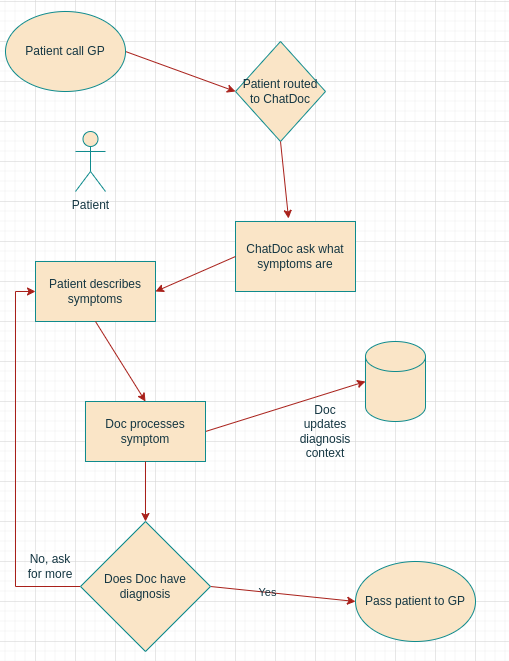
\includegraphics[scale=0.5]{PatientFlow}
\end{center}
This is an approach where the chatbot asks more questions until it can work out a diagnosis. 
This could be used in many other scenarios like trying to find out what is wrong with a engine or to discover what drainage problems on a farm and why. If the chatbot has the right training then there is no limit to where the chatbot can do this. This like what we saw in previously where chatbots are used to work out why things go wrong\cite{gyan}\cite{devops}

\subsection{Bot can take action on behalf of patient like making a booking}
This action is very much like a basic receptionist job. It is easy to automate repetitive and well defined action such as setting up a meeting or requesting a repeat prescription, and this can also shorten waiting times for customers as they are dealt with quickly and will never be in the queue infront of other customers. This ties in very well with the booking prior art we saw previously. Arguably as this is so simple and it seems like there are many other companies already doing this, that it is already a crowded market and if we were to repurpose our chatbot to automate these admin tasks then we would need to find something more advanced or more niche to be of any use.

\subsection{Bot can be empathetic / Bot may be seen as soulless}
We were scared that bots were not empathetic but have seen it turns out that chatbots by their design come across as very empathetic \cite{bedside}. A chatbot that understands patients medical needs and also seems empathetic and has infinite patience lends could work in therapy and psychology. With the correct monitoring in place it could be a very powerful tool. 

\subsection{Bot may make incorrect diagnosis and as such needs to be monitored / Bot may remove certain jobs, and those employees may not be able to or unwilling to retrain}
These were two weaknesses are not helpful.

\section{Alternative business sectors}
Based on our research we can work out what business sectors and which features of our chatbot could be repurposed.

\subsection{Engineering}
All engineering involves problem solving, where engines and machines will malfunction. Working on the symptoms that an engineer is seeing they will want to know what the actual fault is and how to repair that fault. 

\subsubsection{Feature used}
That is the same as our chat bot where a patient talks about symptoms and the chatbot has to work out what is wrong with the patient. The process  in \ref{diagnose} along with the AI processing capabilities could easily be repurposed to diagnose the root cause of issues in engineering disciplines like
\begin{itemize}
    \item Vehicle mechanics
    \item Office electricians
    \item Plumbing and electrics
\end{itemize}
It would mean that anywhere that this feature would be repurposed would need to be retrained on those engines.

\subsection{Theatre bookings}
In \ref{booking} "Finair launched its first chatbot ... it can sell flight" \cite{booking}. Our chatbot can make a booking with a GP. To be able to do this it knows when a GP is free and  this is the same as how Finair was able to sell flights with a chatbot. 
\subsubsection{Feature used}
Making bookings. If our chat bot can make a booking for a GP, then this could be repurposed to making a booking for a Theatre, School plays, Bands, Cinema, Dog kennels.
Anywhere a booking can be made our chatbot can do it instead and make it easy for a customer to work with the chatbot to reserve a date. The only thing that would need to change is that the chatbot would need to be able to take money for tickets but that's for the business to solve.

\bibliography{bibliography}
\end{document}
